\chapter{Kristallografie en röntgendiffractie}\label{ch:b3:x-ray-diffraction}

In 1912 liet een bundel röntgenstralen die door een kristal van
kopersulfaat werd gestuurd, op een fotografische plaat een patroon van
scherpe vlekken achter: kristallen buigen röntgenstraling af zoals een
tralie licht afbuigt, omdat de afstanden tussen hun atomen vergelijkbaar
zijn met de golflengte van röntgenstraling. Een jaar later las William
Lawrence Bragg, toen nog student, uit zulke patronen de structuur van
steenzout af --- en toonde hij aan dat de vaste stof helemaal geen
\ce{NaCl}-moleculen bevat, alleen een rooster waarin elk ion zes buren van
de andere soort heeft. Elke kristalstructuur die in het deel van jaar~1
en in dit boek vermeld wordt, werd op deze manier gevonden. Dit hoofdstuk
geeft de meetkunde van roosters en van hun symmetrie, de voorwaarde voor
diffractie, de intensiteiten die de inhoud van de cel onthullen, en de
poeder- en éénkristalmethoden die in elk laboratorium gebruikt worden.

\begin{recall}
Het deel van jaar~1 beschreef kristallen met een rooster van
roosterpunten, een motief en een eenheidscel met haar roosterparameters;
telde de multipliciteit van een cel; bouwde de kubisch vlakgecentreerde
en kubisch ruimtegecentreerde structuren en de hexagonaal dichtste
stapeling, en de steenzout-, cesiumchloride-, zinkblende- en
fluoriettypes; en berekende een dichtheid uit een cel.
\Cref{ch:b3:point-groups} definieerde \omterm{def:b3:point-groups:operation}{symmetrieoperaties} en \omterm{def:b3:point-groups:point-group}{puntgroepen}.
\end{recall}

\begin{omfigure}
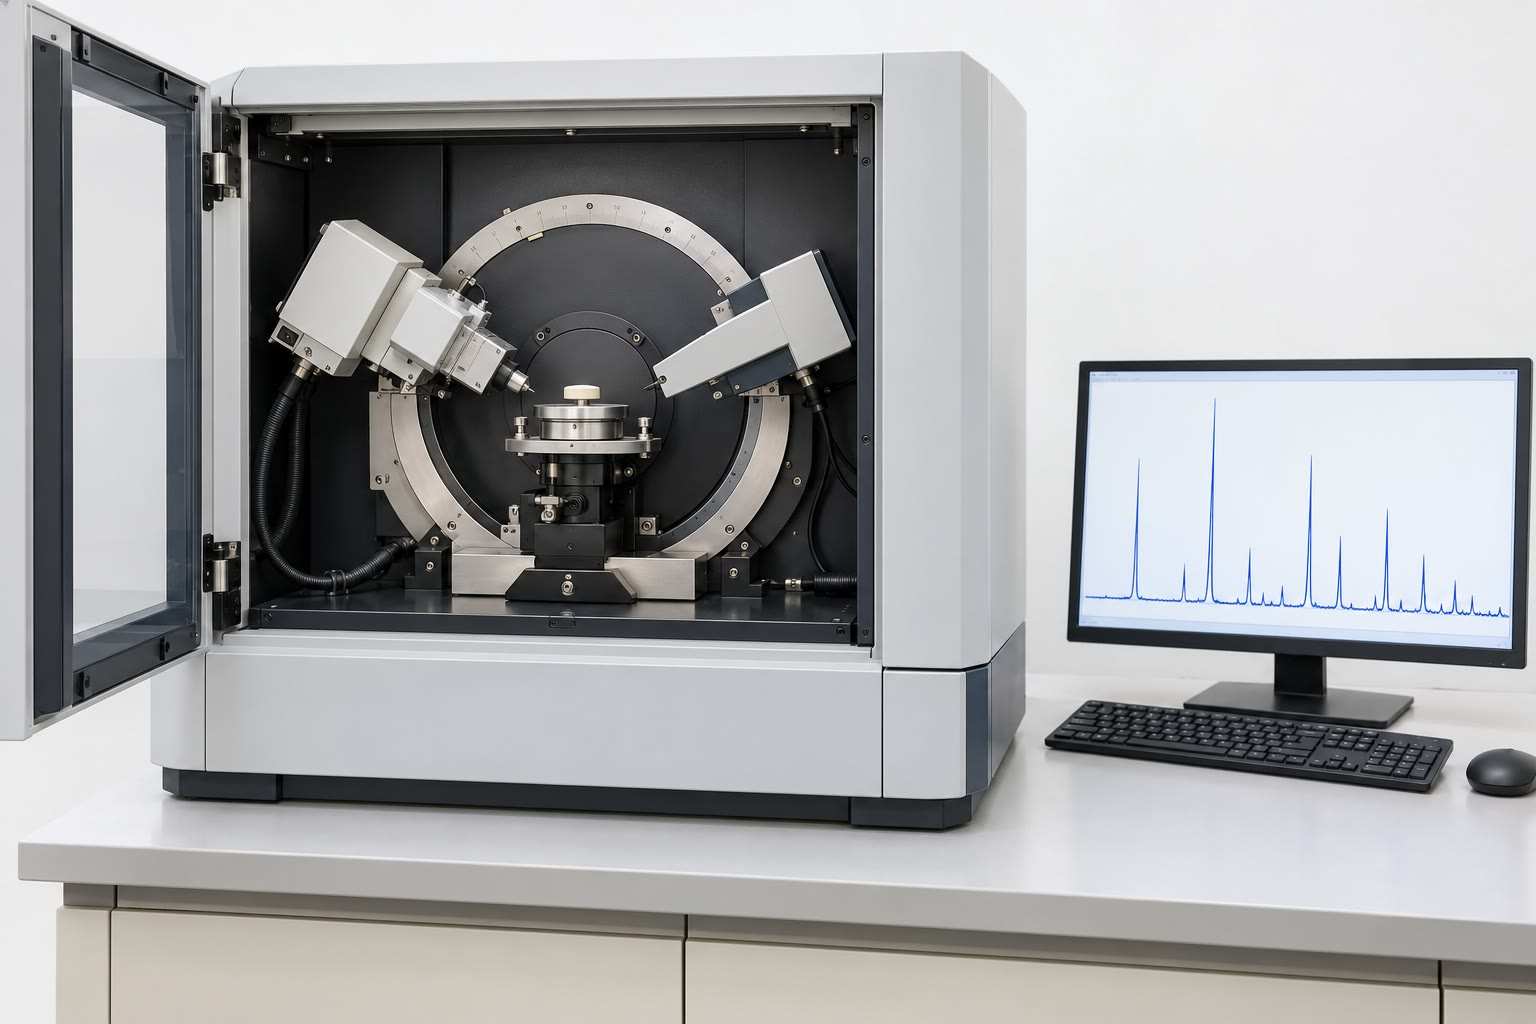
\includegraphics[width=0.6\linewidth]{images/book4/ai/b3-09-diffractometer.jpg}

{\small Een poederdiffractometer voor op de labtafel: de röntgenbuis en de
detector draaien op een cirkel rond het vlakke monster.}
\end{omfigure}

\section{Kristalstelsels en bravaisroosters}

Een rooster kan alleen \omterm{def:b3:point-groups:operation}{symmetrieoperaties} hebben die het rooster op
zichzelf afbeelden. Dat beperkt ze sterk.

\begin{theorem}[De kristallografische beperking]\label{thm:b3:x-ray-diffraction:restriction}
De enige rotatieassen die verenigbaar zijn met een rooster, zijn van orde
1, 2, 3, 4 en 6.
\end{theorem}

\begin{proof}
In een basis van roostervectoren beeldt een symmetrierotatie roostervectoren
af op roostervectoren, zodat haar matrix gehele elementen en een geheel
spoor heeft. Het spoor hangt niet af van de basis; in een orthonormale
basis met $z$ langs de as is het $1 + 2\cos\theta$. Dus is $2\cos\theta$
een geheel getal tussen $-2$ en 2:
$\cos\theta \in \{-1, -\frac12, 0, \frac12, 1\}$, $\theta = 180^\circ, 120^\circ, 90^\circ,
60^\circ, 0^\circ$: ordes 2, 3, 4, 6, 1. Een vijfvoudige as is onmogelijk.
\end{proof}

\begin{definition}[Kristalstelsel, bravaisrooster, roostercentrering]\label{def:b3:x-ray-diffraction:crystal-system}
Roosters worden volgens hun symmetrie ingedeeld in zeven
\emph{kristalstelsels}\index{kristalstelsel} (triklien, monoklien,
orthorombisch, tetragonaal, trigonaal, hexagonaal, kubisch). Een cel kan
alleen roosterpunten op haar hoekpunten hebben (primitief, P), of ook in
haar centrum (ruimtegecentreerd, I), in de middelpunten van alle zijvlakken
(vlakgecentreerd, F) of van één paar zijvlakken (basisgecentreerd, C), of
langs een lichaamsdiagonaal (romboëdrisch, R): dat is haar
\emph{roostercentrering}\index{roostercentrering}. De 14 verschillende
combinaties van een stelsel en een centrering zijn de
\emph{bravaisroosters}\index{bravaisrooster}.
\end{definition}

\begin{center}\small
\begin{tabular}{lll}
\hline
stelsel & voorwaarden voor de cel & centreringen \\ \hline
triklien & geen & P \\
monoklien & $\alpha = \gamma = 90^\circ$ & P, C \\
orthorombisch & $\alpha = \beta = \gamma = 90^\circ$ & P, C, I, F \\
tetragonaal & $a = b$, alle hoeken $90^\circ$ & P, I \\
trigonaal & $a = b = c$, $\alpha = \beta = \gamma \ne 90^\circ$ (romboëdrische assen) & R \\
hexagonaal & $a = b$, $\alpha = \beta = 90^\circ$, $\gamma = 120^\circ$ & P \\
kubisch & $a = b = c$, alle hoeken $90^\circ$ & P, I, F \\ \hline
\end{tabular}
\end{center}

\begin{omfigure}
\tdplotsetmaincoords{60}{100}
\begin{tikzpicture}[tdplot_main_coords, scale=1.25, font=\small]
  \foreach \s/\lab in {0/{kubisch P}, 3.0/{kubisch I}, 6.0/{kubisch F}}{
    \begin{scope}[xshift=\s cm]
      \pic[transform shape] {omcubeo={1.6}};
      \foreach \x in {0,1.6}{\foreach \y in {0,1.6}{\foreach \z in {0,1.6}{\node[cellA=2.6mm] at (\x,\y,\z) {};}}}
      \node[anchor=north] at (0.8,0.8,-0.62) {\lab};
    \end{scope}}
  \begin{scope}[xshift=3.0cm]
    \node[cellB=2.6mm] at (0.8,0.8,0.8) {};
  \end{scope}
  \begin{scope}[xshift=6.0cm]
    \foreach \p in {(0.8,0.8,0),(0.8,0.8,1.6),(0.8,0,0.8),(0.8,1.6,0.8),(0,0.8,0.8),(1.6,0.8,0.8)}{\node[cellB=2.6mm] at \p {};}
  \end{scope}
\end{tikzpicture}

{\small De drie kubische \omterm{def:b3:x-ray-diffraction:crystal-system}{bravaisroosters}: primitief (roosterpunten op de
hoekpunten), ruimtegecentreerd (plus het centrum, rood) en vlakgecentreerd
(plus de zes middelpunten van de zijvlakken, rood). Hun cellen bevatten 1,
2 en 4 roosterpunten.}
\end{omfigure}

\section{Roostervlakken en het reciproke rooster}

\begin{definition}[Roostervlak, millerindices, roostervlakafstand]\label{def:b3:x-ray-diffraction:miller}
Een \emph{roostervlak}\index{roostervlak} is een vlak door minstens drie
niet-collineaire roosterpunten; het behoort tot een familie van
evenwijdige vlakken op gelijke afstanden die alle roosterpunten bevatten.
Als het vlak van de familie dat het dichtst bij de oorsprong ligt de
assen snijdt in $a/h$, $b/k$, $c/l$, dan zijn de gehele getallen $(hkl)$,
zonder gemeenschappelijke factor, zijn
\emph{millerindices}\index{millerindices} (een index 0 voor een vlak
evenwijdig met een as). De afstand tussen naburige vlakken is de
\emph{roostervlakafstand}\index{roostervlakafstand} $d_{hkl}$.
\end{definition}

\begin{proposition}[Afstanden in orthogonale cellen]\label{prop:b3:x-ray-diffraction:spacing}
Voor een orthorombische cel is $\dfrac{1}{d_{hkl}^2} = \dfrac{h^2}{a^2} + \dfrac{k^2}{b^2} +
\dfrac{l^2}{c^2}$; voor een kubische cel is $d_{hkl} = a/\sqrt{h^2 + k^2 + l^2}$.
\end{proposition}

\begin{proof}
Het vlak $hx/a + ky/b + lz/c = 1$ heeft de normaalvector $\mathbf n = (h/a, k/b, l/c)$
en ligt op afstand $1/|\mathbf n|$ van de oorsprong; het evenwijdige vlak
door de oorsprong behoort tot de familie, dus $d = 1/|\mathbf n|$.
\end{proof}

\begin{definition}[Reciprook rooster]\label{def:b3:x-ray-diffraction:reciprocal}
Voor een rooster met basisvectoren $\mathbf a$, $\mathbf b$, $\mathbf c$ en celvolume $V$
heeft het \emph{reciproke rooster}\index{reciprook rooster} de basisvectoren
$\mathbf a^* = (\mathbf b\times\mathbf c)/V$, $\mathbf b^* = (\mathbf c\times\mathbf a)/V$,
$\mathbf c^* = (\mathbf a\times\mathbf b)/V$, zodat $\mathbf a\cdot\mathbf a^* = 1$ en
$\mathbf a\cdot\mathbf b^* = 0$. Zijn roosterpunt $\mathbf G_{hkl} = h\mathbf a^* + k\mathbf b^* + l\mathbf c^*$ staat
loodrecht op de vlakken $(hkl)$, en $|\mathbf G_{hkl}| = 1/d_{hkl}$.
\end{definition}

\section{Diffractie}

\begin{theorem}[Wet van Bragg]\label{thm:b3:x-ray-diffraction:bragg}
Röntgenstralen met golflengte $\lambda$ worden door een familie vlakken
met afstand $d$ alleen gereflecteerd onder de glanshoeken $\theta$ die
voldoen aan
\[
2d\sin\theta = n\lambda, \qquad n = 1, 2, \dots,
\]
de \emph{wet van Bragg}\index{wet van Bragg}. De orde $n$ wordt verwerkt
door de reflectie te schrijven als $(nh\,nk\,nl)$ met afstand $d/n$.
\end{theorem}

\begin{proof}
Stralen die door twee naburige vlakken verstrooid worden, onder gelijke
hoeken van inval en reflectie $\theta$, verschillen in weglengte met $2d\sin\theta$ (de twee
segmenten aan weerszijden van de normaal door het onderste vlak). Ze
versterken elkaar wanneer dat verschil een geheel aantal golflengten is;
met miljoenen vlakken geeft elke andere hoek stralen die elkaar paarsgewijs
uitdoven.
\end{proof}

\begin{omfigure}
\begin{tikzpicture}[font=\small, >=Stealth]
  \foreach \y in {0,-1.1}{\draw[thick] (-0.4,\y) -- (7.4,\y);}
  \foreach \x in {0,1.4,...,7.0}{\fill (\x,0) circle (1.5pt) (\x,-1.1) circle (1.5pt);}
  \draw[->, omDef, thick] (0.2,1.75) -- (2.8,0);
  \draw[->, omDef, thick] (2.8,0) -- (5.4,1.75);
  \draw[->, omDef, thick] (-1.43,1.75) -- (2.8,-1.1);
  \draw[->, omDef, thick] (2.8,-1.1) -- (7.03,1.75);
  \draw[densely dashed] (2.8,0) -- (2.8,-1.1);
  \draw[omThm, thick] (2.8,0) -- (2.18,-0.68) (2.8,0) -- (3.42,-0.68);
  \draw[omThm, very thick] (2.18,-0.68) -- (2.8,-1.1) -- (3.42,-0.68);
  \draw (1.8,0) arc[start angle=180, end angle=213.9, radius=1.0];
  \node[anchor=east] at (1.85,-0.2) {$\theta$};
  \draw[<->] (7.7,0) -- (7.7,-1.1) node[midway, right] {$d$};
  \node[omThm, anchor=north] at (2.8,-1.2) {wegverschil $2d\sin\theta$};
\end{tikzpicture}

{\small De constructie van Bragg. Stralen die door naburige vlakken
gereflecteerd worden, leggen een langere weg af, gelijk aan de twee rode
segmenten van elk $d\sin\theta$; de golven versterken elkaar wanneer
$2d\sin\theta$ een geheel aantal golflengten is.}
\end{omfigure}

\begin{proposition}[Voorwaarde van Laue]\label{prop:b3:x-ray-diffraction:laue}
Met de golfvectoren $\mathbf k$ en $\mathbf k'$ van de invallende en de
verstrooide golf, met lengte
$1/\lambda$, treedt diffractie op wanneer $\mathbf k' - \mathbf k = \mathbf G_{hkl}$, een vector van het
\omterm{def:b3:x-ray-diffraction:reciprocal}{reciproke rooster}; dit is gelijkwaardig met de \omterm{thm:b3:x-ray-diffraction:bragg}{wet van Bragg}.
\end{proposition}

\begin{proof}
Golven die verstrooid worden door twee roosterpunten die een roostervector
$\mathbf R$ uit elkaar liggen, verschillen in fase met $2\pi(\mathbf k' - \mathbf k)\cdot\mathbf R$; ze versterken
elkaar allemaal als dit een veelvoud van $2\pi$ is
voor elke $\mathbf R$, dus als $\mathbf k' - \mathbf k$ tot het \omterm{def:b3:x-ray-diffraction:reciprocal}{reciproke
rooster} behoort (volgens de
definitie $\mathbf a\cdot\mathbf a^* = 1$, $\mathbf a\cdot\mathbf b^* = 0$\dots). Voor elastische verstrooiing is
$|\mathbf k| = |\mathbf k'|$ en $|\mathbf k' - \mathbf k| = 2\sin\theta/\lambda$, waarin $2\theta$ de hoek
ertussen is; met $|\mathbf G| = 1/d$ is dit $2d\sin\theta = \lambda$, en $\mathbf G$ staat loodrecht op
de reflecterende vlakken.
\end{proof}

\begin{definition}[Bol van Ewald]\label{def:b3:x-ray-diffraction:ewald}
De \emph{bol van Ewald}\index{bol van Ewald} heeft straal $1/\lambda$ en gaat
door de oorsprong van het \omterm{def:b3:x-ray-diffraction:reciprocal}{reciproke rooster}, met zijn middelpunt op $-\mathbf k$ van de oorsprong; een
reflectie treedt op telkens wanneer een punt van het \omterm{def:b3:x-ray-diffraction:reciprocal}{reciproke rooster}
erop ligt.
\end{definition}

\begin{omfigure}
\begin{tikzpicture}[font=\small, >=Stealth, scale=0.9]
  \foreach \i in {-2,...,4}{\foreach \j in {-2,...,2}{\fill[black!60] (\i*1.0,\j*0.75) circle (1.3pt);}}
  \node[anchor=north east] at (0,0) {$O$};
  \draw[omDef] (-1.625,0.0) circle (1.625);
  \draw[->, omDef, thick] (-1.625,0) -- (0,0) node[midway, below] {$\mathbf k$};
  \draw[->, omThm, thick] (-1.625,0) -- (-1.0,1.5);
  \node[omThm, anchor=east] at (-1.4,0.85) {$\mathbf k'$};
  \draw[->, black, very thick] (0,0) -- (-1.0,1.5) node[pos=0.3, left] {$\mathbf G$};
  \node[anchor=north] at (-1.625,-1.75) {bol van Ewald, straal $1/\lambda$};
  \draw[<->] (4.6,0) -- (4.6,0.75) node[midway, right] {$b^*$};
  \draw[<->] (3,-1.85) -- (4,-1.85) node[midway, below] {$a^*$};
\end{tikzpicture}

{\small De constructie van Ewald in twee dimensies (de cirkel gaat door de
oorsprong $O$ van het \omterm{def:b3:x-ray-diffraction:reciprocal}{reciproke rooster}). Een roosterpunt $\mathbf G$ op de
cirkel geeft een
afgebogen bundel $\mathbf k' = \mathbf k + \mathbf G$. Hier gaat de cirkel,
met een straal die voor de tekening gekozen is, door het roosterpunt $(-1, 2)$.}
\end{omfigure}

\section{Intensiteiten en symmetrie}

De \omterm{thm:b3:x-ray-diffraction:bragg}{wet van Bragg} geeft de richtingen van de afgebogen bundels, die alleen
van het rooster afhangen; hun intensiteiten hangen af van wat zich in de
cel bevindt.

\begin{definition}[Atomaire verstrooiingsfactor, structuurfactor]\label{def:b3:x-ray-diffraction:structure-factor}
De \emph{atomaire verstrooiingsfactor}\index{atomaire verstrooiingsfactor}
$f_j$ van een atoom is de amplitude die het verstrooit, in eenheden van
die van één elektron; ze is gelijk aan zijn aantal elektronen in de
voorwaartse richting en neemt af bij grotere hoeken. De
\emph{structuurfactor}\index{structuurfactor} van de reflectie $hkl$ is
\[
F_{hkl} = \sum_jf_j\,\eu^{2\pi\iu(hx_j + ky_j + lz_j)},
\]
gesommeerd over de atomen van de cel met fractionele coördinaten $(x_j, y_j, z_j)$.
\end{definition}

\begin{proposition}[Intensiteit]\label{prop:b3:x-ray-diffraction:intensity}
De intensiteit van een reflectie is evenredig met $|F_{hkl}|^2$.
\end{proposition}

\begin{proof}[Gedeeltelijk bewijs]
Atoom $j$ zit op $\mathbf r_j = x_j\mathbf a + y_j\mathbf b + z_j\mathbf c$; voor een reflectie is
$(\mathbf k' - \mathbf k)\cdot\mathbf r_j = hx_j + ky_j + lz_j$, zodat zijn golf de fase
$2\pi(hx_j + ky_j + lz_j)$ heeft ten opzichte van een atoom in de
oorsprong, en de amplitude $f_j$:
de cel verstrooit de som $F_{hkl}$, en elke cel hetzelfde. Een intensiteit
is het kwadraat van de modulus van een amplitude. Dat meervoudige
verstrooiing verwaarloosd mag worden (de kinematische benadering), wordt
hier aangenomen.
\end{proof}

\begin{definition}[Systematische uitdoving]\label{def:b3:x-ray-diffraction:absence}
Een \emph{systematische uitdoving}\index{systematische uitdoving} is een
reflectie waarvan de
\omterm{def:b3:x-ray-diffraction:structure-factor}{structuurfactor} nul is voor elk kristal met een gegeven \omterm{def:b3:x-ray-diffraction:crystal-system}{roostercentrering}
of symmetrie, wat zijn atomen ook zijn.
\end{definition}

\begin{proposition}[Uitdovingen van gecentreerde roosters]\label{prop:b3:x-ray-diffraction:absences}
In een ruimtegecentreerd rooster ontbreken de reflecties met $h + k + l$
oneven; in een vlakgecentreerd rooster ontbreken de reflecties waarvan
$h$, $k$, $l$ gemengde pariteit hebben.
\end{proposition}

\begin{proof}
Centrering I: elk atoom op $(x,y,z)$ heeft een kopie op $(x + \frac12, y + \frac12, z + \frac12)$,
waarvan de fasefactor verschilt met $\eu^{\iu\pi(h+k+l)} = (-1)^{h+k+l}$: $F = (1 +
(-1)^{h+k+l})F'$. Centrering F: kopieën op drie middelpunten van zijvlakken
geven de factor $1 +
(-1)^{h+k} + (-1)^{h+l} + (-1)^{k+l}$, gelijk aan 4 als $h$, $k$, $l$ alle even
of alle oneven zijn, en anders gelijk aan 0.
\end{proof}

\begin{example}[Steenzout en sylviet]\label{ex:b3:x-ray-diffraction:nacl-kcl}
% ledger: lat:NaCl, lat:KCl
In de steenzoutstructuur, met kationen op $(0,0,0)$ en anionen op $(\frac12,0,0)$, elk
met de translaties van F: $F_{hkl} = 4[f_+ + f_-(-1)^{h+k+l}]$ voor
ongemengde indices.
Voor \ce{NaCl} is $f(\ce{Na+}) \approx 10$ en $f(\ce{Cl-}) \approx 18$: de
reflecties met alle indices oneven,
(111), (311), zijn zwak maar aanwezig. Voor \ce{KCl} hebben \ce{K+} en
\ce{Cl-} beide 18
elektronen: de reflecties met alle indices oneven verdwijnen bijna, en het
patroon lijkt op dat van een primitief kubisch rooster met de halve
celribbe (figuur hieronder).
\end{example}

\begin{omfigure}
\begin{tikzpicture}
\begin{axis}[name=salts, width=0.95\linewidth, height=5.2cm, xmin=20, xmax=90,
  ymin=0, ymax=2.55, ytick=\empty, axis x line=bottom, axis y line=none,
  xlabel={$2\theta$ / graad (Cu K$\alpha_1$)}, tick label style={font=\small},
  label style={font=\small}]
\addplot[omDef, thin] table[x=tt, y expr=\thisrow{NaCl}+1.35] {figdata/out/bachelor-3-xrd-powder-salts.dat};
\addplot[omThm, thin] table[x=tt, y=KCl] {figdata/out/bachelor-3-xrd-powder-salts.dat};
\node[font=\small, omDef, anchor=west] at (axis cs:79,1.9) {\ce{NaCl}};
\node[font=\small, omThm, anchor=west] at (axis cs:77,0.55) {\ce{KCl}};
\node[font=\scriptsize, anchor=south] at (axis cs:27.36,1.52) {111};
\node[font=\scriptsize, anchor=west] at (axis cs:32.1,2.25) {200};
\node[font=\scriptsize, anchor=west] at (axis cs:28.8,0.9) {200};
\node[font=\scriptsize, anchor=west] at (axis cs:41.0,0.85) {220};
\end{axis}
\end{tikzpicture}

\begin{tikzpicture}
\begin{axis}[name=met, width=0.62\linewidth, height=4.4cm, xmin=35, xmax=100,
  ymin=0, ymax=2.35, ytick=\empty, axis x line=bottom, axis y line=none,
  xlabel={$2\theta$ / graad}, tick label style={font=\small}, label style={font=\small}]
\addplot[omDef, thin] table[x=tt, y expr=\thisrow{Cu}+1.2] {figdata/out/bachelor-3-xrd-powder-metals.dat};
\addplot[omThm, thin] table[x=tt, y=W] {figdata/out/bachelor-3-xrd-powder-metals.dat};
\node[font=\small, omDef, anchor=west] at (axis cs:55,1.5) {Cu (F)};
\node[font=\small, omThm, anchor=west] at (axis cs:44,0.4) {W (I)};
\end{axis}
\begin{axis}[at={(met.east)}, anchor=west, xshift=0.7cm, width=0.36\linewidth, height=4.4cm,
  xmin=29.7, xmax=33.7, ymin=0, ymax=1.1, ytick=\empty, axis x line=bottom,
  axis y line=none, xlabel={$2\theta$ / graad}, tick label style={font=\small},
  label style={font=\small}, title={\small Scherrer}]
\addplot[black, thick] table[x=tt, y=L200] {figdata/out/bachelor-3-xrd-powder-scherrer.dat};
\addplot[omDef, thick] table[x=tt, y=L50] {figdata/out/bachelor-3-xrd-powder-scherrer.dat};
\addplot[omThm, thick] table[x=tt, y=L10] {figdata/out/bachelor-3-xrd-powder-scherrer.dat};
\end{axis}
\end{tikzpicture}

{\small Berekende poederdiffractogrammen (Cu K$\alpha_1$; verstrooiingsfactoren
gelijk genomen aan het aantal elektronen, zodat alleen de uitdovingen en
de grote tendensen van de intensiteit betekenis hebben). Boven: \ce{NaCl}
en \ce{KCl}; de lijnen van \ce{KCl} met alle indices oneven verdwijnen.
Linksonder: koper (F) vertoont (111), (200), (220), (311)\dots; wolfraam
(I) vertoont (110), (200), (211)\dots. Rechtsonder: de lijn (200) van
\ce{NaCl} voor kristallieten van 200 (zwart), 50 (blauw) en 10 nm (rood):
kleinere kristallen geven bredere lijnen.}
\end{omfigure}

\begin{proposition}[Wet van Friedel]\label{prop:b3:x-ray-diffraction:friedel}
Zonder anomale verstrooiing is $|F_{hkl}| = |F_{\bar h\bar k\bar l}|$: een
diffractiepatroon ziet er centrosymmetrisch uit, zelfs wanneer het kristal
dat niet is.
\end{proposition}

\begin{proof}
Met reële $f_j$ is $F_{\bar h\bar k\bar l} = \sum f_j\eu^{-2\pi\iu(\dots)} = F_{hkl}^*$, met dezelfde
modulus.
\end{proof}

\omterm{def:b3:point-groups:operation}{Symmetrie-elementen} die een rotatie of een spiegeling combineren met een
fractie van een roostertranslatie, bestaan alleen in kristallen.

\begin{definition}[Schroefas, glijspiegelvlak, ruimtegroep]\label{def:b3:x-ray-diffraction:space-group}
Een \emph{schroefas}\index{schroefas} $n_p$ combineert een rotatie over $2\pi/n$ met een
translatie over $p/n$ van de roosterperiode langs de as ($2_1$: een halve
draai en een halve cel). Een \emph{glijspiegelvlak}\index{glijspiegelvlak}
combineert een spiegeling met een translatie over een halve roostervector
evenwijdig met het vlak ($a$-, $b$-, $c$-glijspiegeling).
De groep van alle \omterm{def:b3:point-groups:operation}{symmetrieoperaties} van een kristal, translaties
inbegrepen, is zijn \emph{ruimtegroep}\index{ruimtegroep}: er zijn er 230.
Het kleinste deel ervan waaruit het hele kristal door de operaties
gegenereerd wordt, is de
\emph{asymmetrische eenheid}\index{asymmetrische eenheid}. Een verzameling
punten die door een \omterm{def:b3:point-groups:class}{ondergroep} van de operaties op zichzelf afgebeeld
wordt, is een
\emph{wyckoffpositie}\index{wyckoffpositie}: algemene posities hebben geen
symmetrie, speciale posities liggen op \omterm{def:b3:point-groups:operation}{symmetrie-elementen}.
\end{definition}

\begin{proposition}[Uitdovingen door een schroefas]\label{prop:b3:x-ray-diffraction:screw-absence}
Een as $2_1$ langs $b$ doet de reflecties $0k0$ met $k$ oneven uitdoven.
\end{proposition}

\begin{proof}
De as beeldt $(x, y, z)$ af op $(-x, y + \frac12, -z)$. Voor $h = l = 0$
hebben beide atomen de fasefactoren $\eu^{2\pi\iu ky}$ en $\eu^{2\pi\iu k(y + 1/2)} = (-1)^k\eu^{2\pi\iu ky}$: hun som
is nul voor oneven $k$.
\end{proof}

\begin{method}[Het symbool van een ruimtegroep lezen]\label{met:b3:x-ray-diffraction:read-space-group}
\begin{enumerate}
  \item De eerste letter is de \omterm{def:b3:x-ray-diffraction:crystal-system}{roostercentrering} (P, I, F, C, R).
  \item De volgende symbolen geven de symmetrie langs de hoofdrichtingen;
        voor het monokliene stelsel is de enige richting $b$. Een breukstreep
        betekent ``met een vlak loodrecht op deze as''.
  \item \textit{P}$2_1/c$, de meest voorkomende \omterm{def:b3:x-ray-diffraction:space-group}{ruimtegroep} van organische
        moleculen: primitief, een as $2_1$ langs $b$, en een
        $c$-glijspiegelvlak loodrecht daarop; samen brengen ze
        inversiecentra voort. Uitdovingen: $0k0$ met $k$ oneven, $h0l$ met $l$
        oneven.
\end{enumerate}
\end{method}

\begin{omfigure}
\begin{tikzpicture}[x=3.6cm, y=3.6cm, font=\small]
  \draw (0,0) rectangle (1,1);
  \node[anchor=north] at (0.5,-0.05) {$a \rightarrow$};
  \node[anchor=east] at (-0.05,0.5) {$b \uparrow$};
  % c-glide planes perpendicular to b at y = 1/4 and 3/4 (glide along c, normal to the page): dotted
  \draw[black, line width=1.1pt, dotted] (0,0.25) -- (1,0.25) (0,0.75) -- (1,0.75);
  % 2_1 axes parallel to b at x = 0, 1/2, 1 (height z = 1/4): lines with half-arrowheads
  \foreach \x in {0,0.5,1}{
    \draw[black, line width=1pt, {Straight Barb[left]}-{Straight Barb[left]}] (\x,0.03) -- (\x,0.97);}
  \node[font=\scriptsize, anchor=west] at (0.51,0.88) {$\tfrac14$};
  % centres of inversion at the corners, edge midpoints and centre
  \foreach \p in {(0,0),(0.5,0),(1,0),(0,0.5),(0.5,0.5),(1,0.5),(0,1),(0.5,1),(1,1)}{\pic at \p {ominv};}
  % general positions: (x,y,z), (-x,y+1/2,1/2-z), (-x,-y,-z), (x,1/2-y,1/2+z)
  \pic at (0.20,0.10) {omgenpos={$+$}{0}};
  \pic at (0.80,0.60) {omgenpos={$\tfrac12{-}$}{0}};
  \pic at (0.80,0.90) {omgenpos={$-$}{1}};
  \pic at (0.20,0.40) {omgenpos={$\tfrac12{+}$}{1}};
\end{tikzpicture}

{\small De \omterm{def:b3:x-ray-diffraction:space-group}{ruimtegroep} \textit{P}$2_1/c$ gezien langs $c$ (projectie op het
$ab$-vlak). Gestippelde lijnen: $c$-glijspiegelvlakken loodrecht op $b$;
halve pijlen: schroefassen $2_1$
langs $b$ (op hoogte $z = \frac14$); kleine cirkels: inversiecentra. Een
algemene positie op hoogte $+z$ genereert er drie andere; een komma geeft
een spiegelbeeldige kopie aan (voortgebracht door de glijspiegeling of de
inversie); $\frac12{-}$ betekent hoogte $\frac12 - z$.}
\end{omfigure}

\section{Poeder- en éénkristalmethoden}

\begin{definition}[Poederdiffractogram]\label{def:b3:x-ray-diffraction:powder}
Een fijngemalen monster bevat kristallieten in alle oriëntaties: elke
familie vlakken vindt er enkele in reflecterende stand, en de afgebogen
bundels vormen kegels. De intensiteit die als functie van $2\theta$
geregistreerd wordt, is het
\emph{poederdiffractogram}\index{poederdiffractogram}, een vingerafdruk
van de kristallijne fase.
\end{definition}

\begin{method}[Een kubisch poederdiffractogram indiceren]\label{met:b3:x-ray-diffraction:index-cubic}
\begin{enumerate}
  \item Bereken $\sin^2\theta$ voor elke lijn; voor een kubisch kristal is $\sin^2\theta =
        (\lambda^2/4a^2)N$ met $N = h^2 + k^2 + l^2$.
  \item Deel door de kleinste waarde en zoek de reeks gehele getallen: P geeft
        $N = 1, 2, 3, 4, 5, 6, 8, \dots$ (nooit 7); I geeft $2, 4, 6, 8, 10, \dots$; F geeft
        $3, 4, 8, 11, 12, 16, \dots$
  \item Kies de reeks die bij alle lijnen past; dan is $a = \lambda\sqrt N/(2\sin\theta)$, bij
        voorkeur uit lijnen bij grote hoeken, waar een fout in $\theta$ het
        minst doorweegt.
\end{enumerate}
\end{method}

\begin{method}[Het aantal formule-eenheden in de cel]\label{met:b3:x-ray-diffraction:z-from-density}
Met de molaire massa $M$ van een formule-eenheid en de gemeten dichtheid $\rho$ moet $Z =
\rho N_Aa^3/M$ (voor een kubische cel) een geheel getal zijn; dat toetst
een voorgestelde structuur.
\end{method}

\begin{proposition}[Vergelijking van Scherrer]\label{prop:b3:x-ray-diffraction:scherrer}
Kristallieten met een gemiddelde grootte $L$ verbreden een lijn met $\beta \approx K\lambda/(L\cos\theta)$ (volle
breedte op halve hoogte in radialen van $2\theta$, $K \approx 0.9$).
\end{proposition}
\admitted

Onder ongeveer \qty{100}{nm} wordt de verbreding meetbaar; de vergelijking
van Scherrer, in meer gevorderde cursussen afgeleid uit de
fouriergetransformeerde van een eindige stapel vlakken, schat dan de
grootte van nanokristallen (\cref{ch:b3:inorganic-materials}).

\begin{definition}[Faseprobleem, R-factor]\label{def:b3:x-ray-diffraction:refinement}
De intensiteiten geven $|F_{hkl}|$, maar niet de fasen van de $F_{hkl}$;
zonder die fasen kan de \omterm{def:b3:computational-chemistry:dft}{elektronendichtheid} niet berekend worden door de
fourierreeks om te keren. Dit is het
\emph{faseprobleem}\index{faseprobleem}. Een proefstructuur wordt verfijnd
met de kleinstekwadratenmethode tot berekende en waargenomen moduli
overeenstemmen; het residu $R = \sum\big||F_o| - |F_c|\big|/\sum|F_o|$ is haar
\emph{R-factor}\index{R-factor} --- enkele procenten voor een goede
structuur.
\end{definition}

Voor een éénkristal meet een diffractometer duizenden reflecties; directe
methoden (statistische betrekkingen tussen de fasen van sterke reflecties)
geven voor de meeste kleine moleculen een eerste
elektronendichtheidskaart, en de verfijning plaatst elk atoom tot op
enkele duizendsten van een nanometer. De resultaten worden als CIF-bestanden
in open databanken gedeponeerd, waaruit de roosterparameters die in deze
reeks vermeld worden, afkomstig zijn.

\begin{inthelab}[Een poedermeting]
Het poeder wordt fijngewreven in een agaatmortier, plat geperst in een
houder, en gescand van 5 tot \ang{90} in $2\theta$ met Cu
K$\alpha$-straling; een nikkelfilter verwijdert het grootste deel van de
K$\beta$-lijn. Het diffractogram wordt vergeleken met referentiepatronen
uit een databank, en de roosterparameters worden verfijnd met een interne
standaard zoals siliciumpoeder. Röntgentoestellen zijn afgesloten en
beveiligd: de sluiter kan niet open wanneer de deur open is.
\end{inthelab}

\begin{history}[De Braggs, 1913]
\begin{minipage}[t]{0.72\linewidth}
Max von Laue stelde in 1912 voor dat kristallen röntgenstraling afbuigen,
en Walter Friedrich en Paul Knipping registreerden het eerste patroon.
William Lawrence Bragg, tweeëntwintig jaar oud, verklaarde de vlekken als
reflecties op roostervlakken en loste, met zijn vader William Henry Bragg,
die een röntgenspectrometer bouwde, in 1913 de structuren van \ce{NaCl},
\ce{KCl} en diamant op. Vader en zoon deelden de Nobelprijs voor de
Natuurkunde van 1915.
\end{minipage}\hfill
\begin{minipage}[t]{0.22\linewidth}\vspace{0pt}
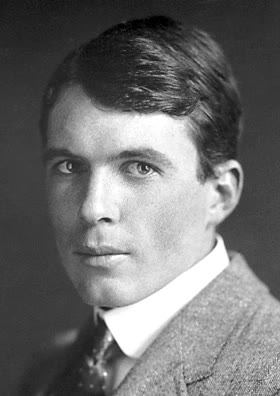
\includegraphics[width=\linewidth]{images/book4/bragg-wl.jpg}\par
{\footnotesize W. L. Bragg.}
\end{minipage}
\end{history}

\section{Oefeningen}

\begin{exercise}[$\star$]\label{exo:b3:x-ray-diffraction:1}
% ledger: lat:NaCl
Bereken voor \ce{NaCl} ($a = \qty{564.06}{pm}$) $d_{111}$, $d_{200}$ en $d_{220}$.
\end{exercise}

\begin{exercise}[$\star$]\label{exo:b3:x-ray-diffraction:2}
% ledger: lat:Cu, xray:CuKa1
Koper is kubisch vlakgecentreerd met $a = \qty{361.50}{pm}$. Benoem met Cu
K$\alpha_1$ ($\lambda = \qty{154.06}{pm}$) de eerste twee reflecties en
bereken hun $2\theta$.
\end{exercise}

\begin{exercise}[$\star$]\label{exo:b3:x-ray-diffraction:3}
Welke van de reflecties 100, 110, 111, 200, 210, 211, 220 zijn aanwezig
voor een kubisch P-, I- en F-rooster?
\end{exercise}

\begin{exercise}[$\star$]\label{exo:b3:x-ray-diffraction:4}
Geef de reciproke basis van een tweedimensionaal rechthoekig rooster met
zijden
$a$ en $b$, en teken de eerste punten van het \omterm{def:b3:x-ray-diffraction:reciprocal}{reciproke rooster}.
\end{exercise}

\begin{exercise}[$\star\star$]\label{exo:b3:x-ray-diffraction:5}
% ledger: lat:W
Een metaal geeft lijnen bij $2\theta = 40.27$, 58.26, 73.20, 87.01 en
\ang{100.66} met Cu
K$\alpha_1$. Indiceer het diffractogram, bepaal het roostertype en $a$.
\end{exercise}

\begin{exercise}[$\star\star$]\label{exo:b3:x-ray-diffraction:6}
% ledger: lat:KCl
Een kristal van \ce{KCl} ($a = \qty{629.29}{pm}$) heeft een gemeten
dichtheid van
\qty{1.99}{g/cm^3} (gegevens van de oefening). Bepaal $Z$.
\end{exercise}

\begin{exercise}[$\star\star$]\label{exo:b3:x-ray-diffraction:7}
De lijn (200) van een \ce{NaCl}-nanopoeder ($2\theta = \ang{31.70}$) is
\ang{0.40} breed, zonder bijdrage van het instrument. Schat de grootte van
de kristallieten.
\end{exercise}

\begin{exercise}[$\star\star$]\label{exo:b3:x-ray-diffraction:8}
\ce{CsCl} heeft \ce{Cs+} op $(0,0,0)$ en \ce{Cl-} op $(\frac12,\frac12,\frac12)$ in een P-cel. Bereken met $f
\approx$ het aantal elektronen $F_{100}$ en $F_{110}$ en de verhouding van
hun intensiteiten (alleen de \omterm{def:b3:x-ray-diffraction:structure-factor}{structuurfactor}). Waarom is \ce{CsCl} niet
ruimtegecentreerd?
\end{exercise}

\begin{exercise}[$\star\star$]\label{exo:b3:x-ray-diffraction:9}
Toon aan dat een C-gecentreerd rooster (extra roosterpunt op $(\frac12,\frac12,0)$) de
reflecties met $h + k$ oneven doet uitdoven.
\end{exercise}

\begin{exercise}[$\star\star\star$]\label{exo:b3:x-ray-diffraction:10}
Leg uit waarom de ontdekking, in de jaren 1980, van legeringen waarvan de
diffractiepatronen scherpe vlekken met tienvoudige symmetrie vertonen, niet
in strijd was met de kristallografische beperking, en wat ze veranderde
aan de definitie van een kristal.
\end{exercise}

\begin{exercise}[$\star\star\star$]\label{exo:b3:x-ray-diffraction:11}
Toon aan dat in \textit{P}$2_1/c$ het \omterm{def:b3:x-ray-diffraction:space-group}{glijspiegelvlak} de reflecties $h0l$ met $l$
oneven doet uitdoven.
\end{exercise}

\begin{exercise}[$\star\star\star$]\label{exo:b3:x-ray-diffraction:12}
Een zuiver enantiomeer kan nooit kristalliseren in een \omterm{def:b3:x-ray-diffraction:space-group}{ruimtegroep} die een
\omterm{def:b3:point-groups:inversion}{inversiecentrum}, een \omterm{def:b3:point-groups:mirror}{spiegelvlak} of een \omterm{def:b3:x-ray-diffraction:space-group}{glijspiegelvlak} bevat. Waarom? Tot
welk soort \omterm{def:b3:x-ray-diffraction:space-group}{ruimtegroepen} is het beperkt, en wat betekent de wet van
Friedel voor de bepaling van zijn absolute configuratie?
\end{exercise}

% keep the heading with its problem box, which fills a page by itself
\clearpage
\enlargethispage{3\baselineskip}
\section{Probleem: welk wit poeder?}

\begin{problem}[{Weekendprobleem --- een poederdiffractogram van een onbekend
kubisch zout: afstanden, indicering, roosterparameter, identiteit en
kristallietgrootte}]
\label{pb:b3:x-ray-diffraction:1}
% ledger: xray:CuKa1, lat:NaCl, lat:KCl, lat:KBr
Een onbekend wit kristallijn poeder, waarvan bekend is dat het \ce{NaCl},
\ce{KCl} of \ce{KBr} is, geeft met Cu K$\alpha_1$-straling ($\lambda = \qty{154.059}{pm}$) de lijnen (gegevens van het
probleem, berekend voor deze oefening):
\begin{center}\small
\begin{tabular}{lcccccc}
\hline
$2\theta$ / graad & 28.342 & 40.512 & 50.178 & 58.632 & 66.380 & 73.692 \\
relatieve intensiteit & 100 & 92 & 38 & 20 & 61 & 49 \\ \hline
\end{tabular}
\end{center}
Er verschijnt geen andere lijn tussen 20 en \ang{75}. Referentiewaarden van
de roosterparameter:
\ce{NaCl} \qty{564.06}{pm}, \ce{KCl} \qty{629.29}{pm}, \ce{KBr} \qty{658.47}{pm}. Molaire massa's:
K 39.1, Na 23.0, Cl 35.5, Br \qty{79.9}{g/mol}.

\medskip\noindent\textbf{Deel I --- Afstanden.}
\begin{enumerate}
  \item Bereken $\theta$ en $d$ voor de eerste lijn.
  \item Bereken $d$ voor alle lijnen.
  \item Bereken de verhoudingen $\sin^2\theta/\sin^2\theta_1$.
  \item Welke reeks gehele getallen vind je?
  \item Kan het een primitief kubisch rooster zijn? Met welke $a$?
  \item Welke $N$ is bij primitief kubisch onmogelijk? Beslist het
        diffractogram al?
\end{enumerate}

\medskip\noindent\textbf{Deel II --- Het echte rooster.}
\begin{enumerate}[resume]
  \item De drie kandidaten hebben alle een F-rooster. Indiceer de lijnen met
        de reeks van F.
  \item Leid $a$ af uit de eerste lijn.
  \item Welke kandidaat past?
  \item Waarom ontbreken voor dat zout de reflecties met alle indices
        oneven, (111) en (311)?
  \item Zou \ce{NaCl} (111) vertonen? En \ce{KBr}?
  \item Leg uit waarom de primitieve interpretatie van Deel I een valkuil is.
\end{enumerate}

\medskip\noindent\textbf{Deel III --- Dichtheid en inhoud.}
\begin{enumerate}[resume]
  \item Hoeveel formule-eenheden bevat de cel?
  \item Bereken de dichtheid uit de cel.
  \item Geef het coördinatiegetal van elk ion.
  \item Bereken de kortste afstand K--Cl.
  \item Welke reflectie zou als eerste boven \ang{75} verschijnen?
  \item Waarom zijn intensiteiten minder bruikbaar dan posities om een fase
        te identificeren?
\end{enumerate}

\medskip\noindent\textbf{Deel IV --- Verfijning en kristallietgrootte.}
\begin{enumerate}[resume]
  \item Waarom berekent men de roosterparameter het best uit een lijn bij
        een grote hoek?
  \item Bereken $a$ uit de lijn (420).
  \item De lijn (420) is \ang{0.25} breed in $2\theta$ (instrumenteel
        verwaarloosbaar); schat de kristallietgrootte.
  \item Zou een kristallietgrootte van \qty{1}{\micro m} de lijn meetbaar
        verbreden?
  \item Formuleer het resultaat: de roosterparameter uit de lijn (420)
        en de identiteit van het poeder.
\end{enumerate}
\end{problem}
